\documentclass{seminar}
\usepackage[display]{texpower}
\usepackage[utf8]{inputenc}
\usepackage{german}
\usepackage{graphicx}
\usepackage{longtable}
\usepackage{hyperref}

%\usepackage[usenames,dvipsnames]{xcolor}
%\definecolor{ueblue}{rgb}{0,0,0.2}
%\definecolor{ueblue}{rgb}{0.6,0.6,1}
%\everymath{\color{yellow}}
%\everydisplay{\color{yellow}}
%\pagecolor{ueblue}
%\pagecolor{ueblue}
%\color{white}

% comment out to have info centered on slides
\centerslidesfalse
\providecommand{\T}[1]{
	\begin{center}
		{\bf #1}
	\end{center}
	\vspace{2mm}
	\hrule
	\vspace{2mm}
}

\newpagestyle{mypagestyle}%
{}%
{http://www.metalab.at \hfil \sl Einführung ins Metalab}


% maketitle
\title{Eine Einführung ins Metalab}
\author{ Hans (aka Zem) Freitag }

\begin{document}

\pagestyle{empty}
\centerslidestrue
\begin{slide}
	\maketitle
	\begin{center}
		Ein Hackspace im Herzen Wiens\\
		{\sf (Rechtschreibfehler sind ein Feature!)}
	\end{center}
\end{slide}
\centerslidesfalse

\pagestyle{mypagestyle}

\begin{slide}
	\T{EinE HackerIn ist\ldots}
	eine experimentierfreudige Personen \ldots \pause
	die mit ihren Fachkenntnissen eine Technologie, beliebiger Art, außerhalb ihrer 
   normalen Zweckbestimmung oder ihres gewöhnlichen Gebrauchs benutzen.
\end{slide}

\begin{slide}
	\T{Ein Hackspace ist\ldots}
	ein physischer, häufig offener Raum, in dem sich HackerInnen und Interessierte treffen 
	und austauschen können. \\ 
\end{slide}

\begin{slide}
	\T{Das Metalab ist\ldots}
	ein unabhängig und gemeinschaftlich betriebener Raum für technisch-kreative 
	Projekte im Zentrum von Wien, gleich hier.
\end{slide}

\begin{slide}
	\T{Typische Aktivitäten eines Hackspaces\ldots}
	\begin{itemize}
		\item Workshops \pause
		\item Öffentlichkeitsarbeit durch Präsentationen, Vorführungen und Vorträge \pause
		\item soziale Aktivitäten wie das Teilen von Wissen und gemeinsames Lernen \pause
		\item die Organisation von Partys und Spielen \pause
	\end{itemize}
\end{slide}

\begin{slide}
	\T{Journalismus Workshop}
	\begin{center}
		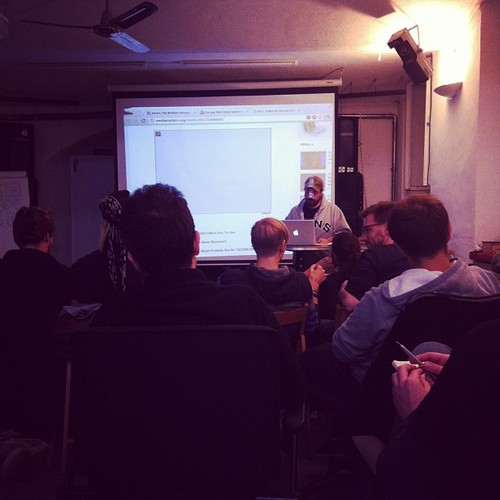
\includegraphics[scale=0.35]{journalism_workshop.jpeg}
	\end{center}
\end{slide}

\begin{slide}
	\T{Zusammenbau von Wareable Electronics}
	\begin{center}
		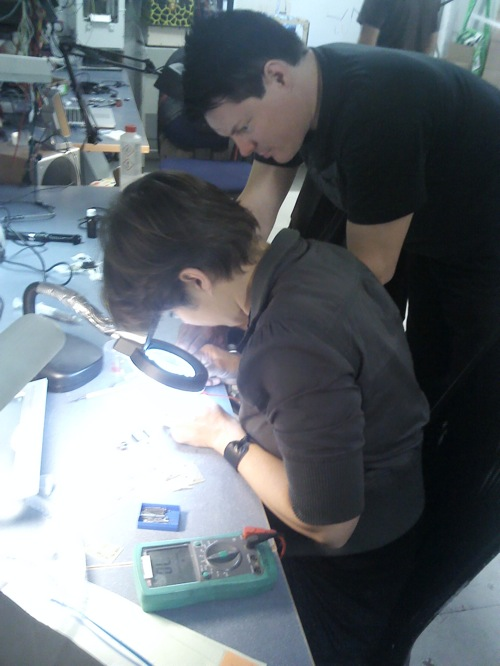
\includegraphics[scale=0.25]{assembly_of_wareable_electronics.jpeg}
	\end{center}
\end{slide}

\begin{slide}
	\T{Softwareentwicklung für Smartphones hier das N9}
	\begin{center}
		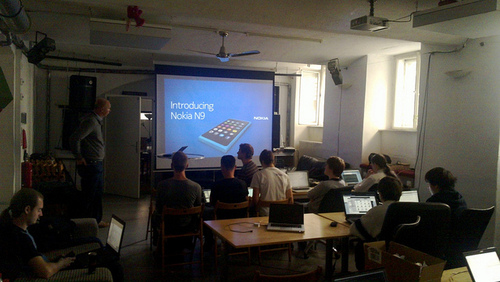
\includegraphics[scale=0.5]{n9_hackaton.jpeg}
	\end{center}
\end{slide}

\begin{slide}
	\T{Robo Flowers}
	\begin{center}
		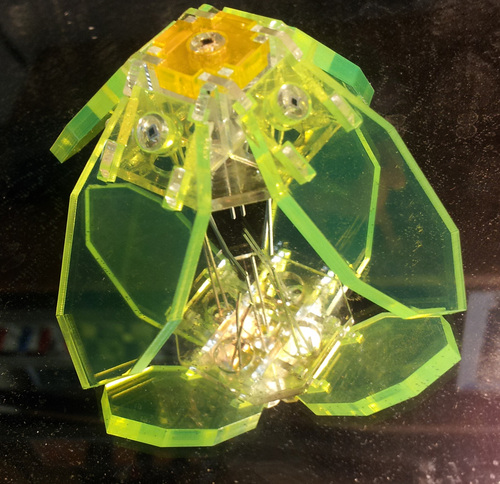
\includegraphics[scale=0.4]{roboflower.jpeg}
	\end{center}
\end{slide}

\begin{slide}
	\T{Dieselbike}
	\begin{center}
		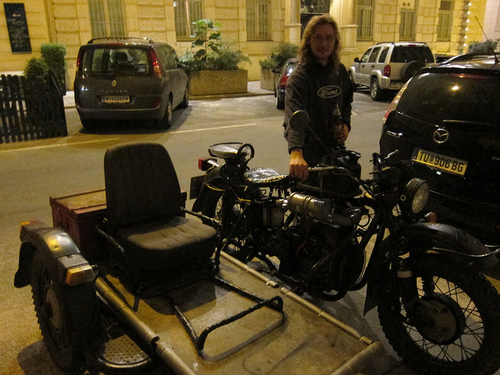
\includegraphics[scale=0.5]{dieselbike.jpeg}
	\end{center}
\end{slide}

\begin{slide}
	\T{Electronik Debugging}
	\begin{center}
		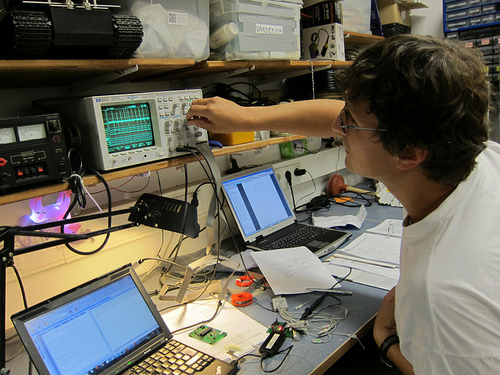
\includegraphics[scale=0.5]{elektronic_debugging.jpeg}
	\end{center}
\end{slide}

\begin{slide}
	\T{Electronik Leiterplatten Herstellung}
	\begin{center}
		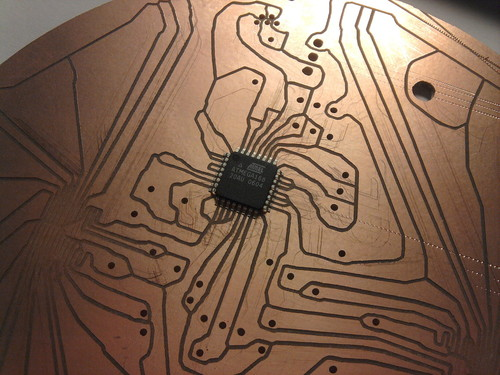
\includegraphics[scale=0.5]{milled_pcb.jpeg}
	\end{center}
\end{slide}

\begin{slide}
	\T{Food Hacking}
	\begin{center}
		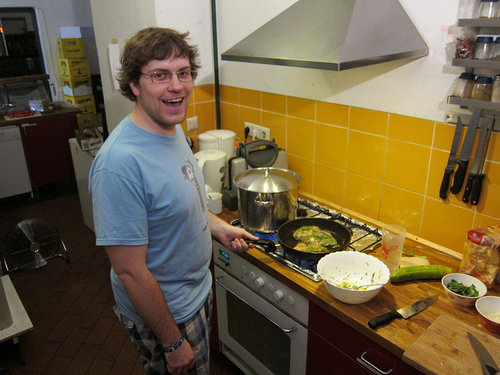
\includegraphics[scale=0.5]{food_hacking.jpeg}
	\end{center}
\end{slide}

\begin{slide}
	\T{3D Printing}
	\begin{center}
		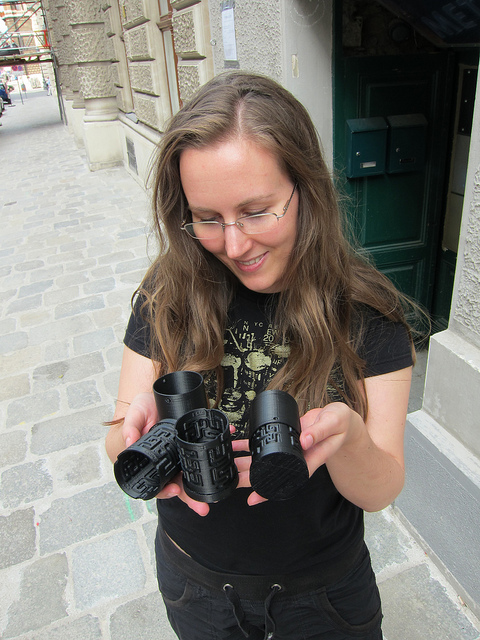
\includegraphics[scale=0.7]{3d-printing.jpeg}
	\end{center}
\end{slide}

\begin{slide}
	\T{3D Printers}
	\begin{center}
		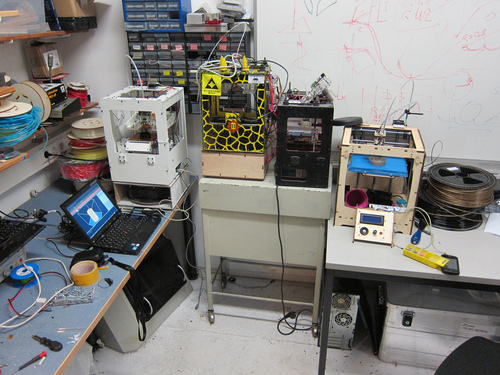
\includegraphics[scale=0.5]{3d_printers.jpeg}
	\end{center}
\end{slide}

\begin{slide}
	\T{Vintage Fotografie}
	\begin{center}
		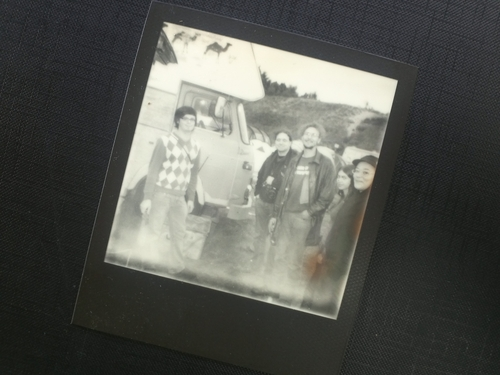
\includegraphics[scale=0.5]{polaroid.jpeg}
	\end{center}
\end{slide}

\begin{slide}
	\T{Camp}
	\begin{center}
		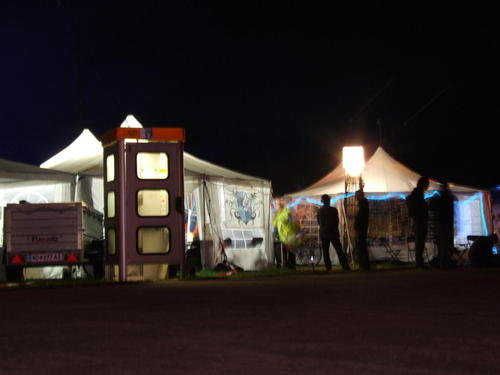
\includegraphics[scale=0.5]{camp.jpeg}
	\end{center}
\end{slide}

\begin{slide}
	\T{Luftmatrazenstöpsel Drucken}
	\begin{center}
		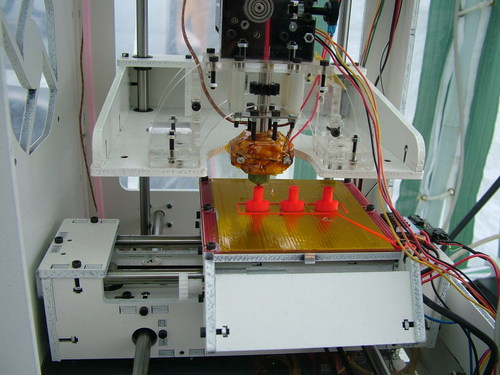
\includegraphics[scale=0.5]{air_matrace_plugs.jpeg}
	\end{center}
\end{slide}

\begin{slide}
	\T{Palatschinkomat}
	\begin{center}
		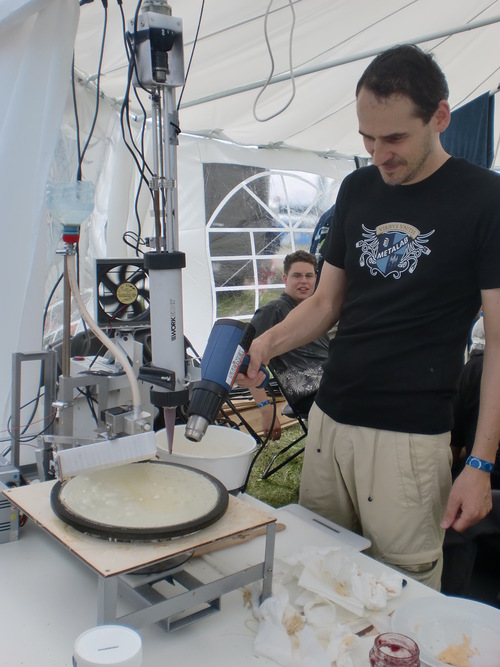
\includegraphics[scale=0.3]{palatschinkomat.jpeg}
	\end{center}
\end{slide}

\begin{slide}
	\T{Umbau eines Fernsehers für ein Kunstprojekt}
	\begin{center}
		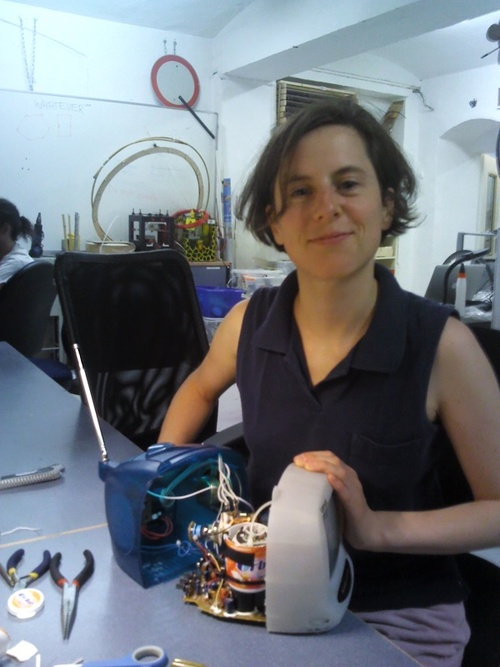
\includegraphics[scale=0.27]{modifying_crt_tv.jpeg}
	\end{center}
\end{slide}

\begin{slide}
	\T{Funkamateure im Metalab}
	\begin{center}
		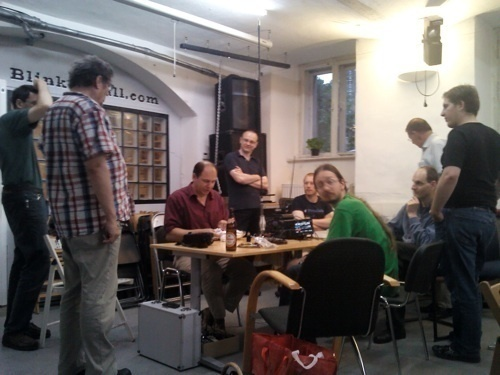
\includegraphics[scale=0.5]{metafunk.jpeg}
	\end{center}
\end{slide}

\begin{slide}
	\T{Seifenblasenmaschine}
	\begin{center}
		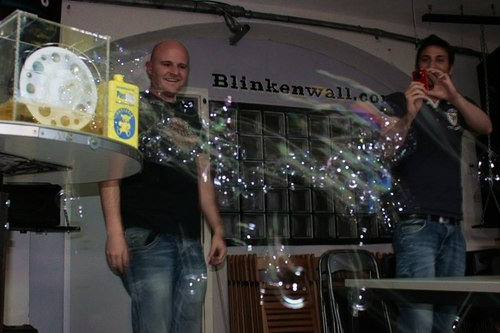
\includegraphics[scale=2]{bubbleomat.jpeg}
	\end{center}
\end{slide}

\begin{slide}
	\T{Selbstgebaute Gitarren}
	\begin{center}
		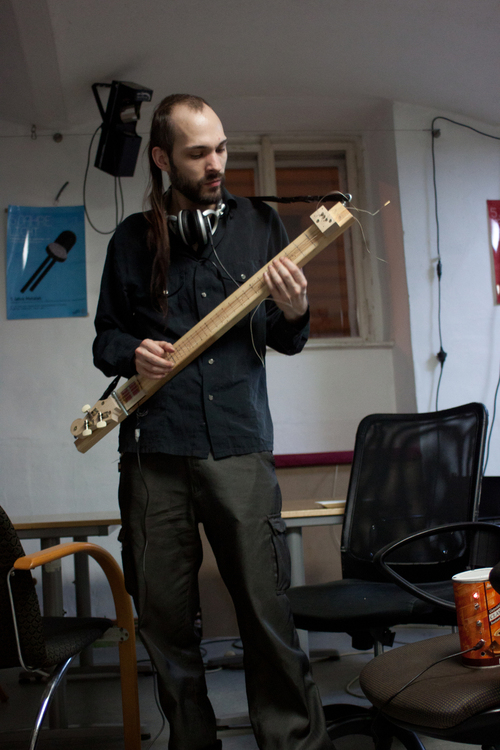
\includegraphics[scale=0.8]{guitars.jpeg}
	\end{center}
\end{slide}

\begin{slide}
	\T{Die Räume des Metalab}
	\begin{itemize}
		\item Hauptraum \pause
		\item Bibliothek \pause
		\item (Audiokammerl zur Zeit leer) \pause
		\item Küche \pause
		\item Lounge (Raucherkammerl) \pause
		\item Whateverlab \pause
		\item Heavylab \pause
		\item Chemlab \pause
		\item Wuzzler 
	\end{itemize}
\end{slide}

\begin{slide}
	\T{Die Räume des Metalab}
	\begin{center}
		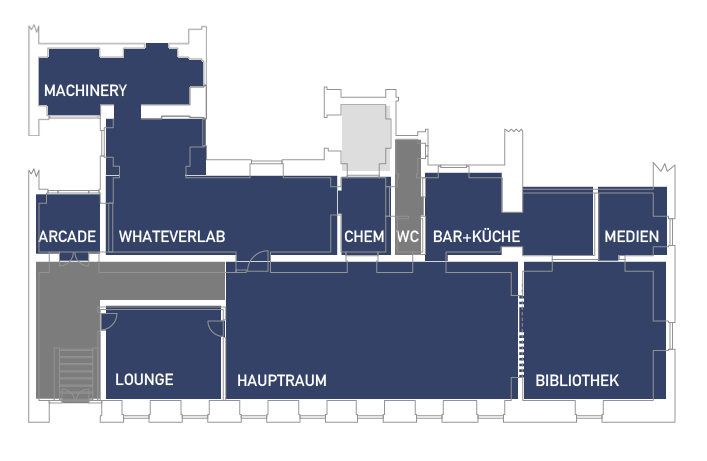
\includegraphics[scale=0.4]{the_lab.png}
	\end{center}
\end{slide}

\begin{slide}
	\T{Ich kenn mich nicht aus, was soll ich hier?}
	\begin{center}
		Wenn wir uns mit allem auskennen würden gäbe es das Metalab nicht! \pause 
		Also, \\
		{\Huge Komm ins Metalab!}
	\end{center}
\end{slide}

\end{document}
